%% VEIN manuscript --- Springer Nature article class (sn-jnl).
%% Author-year reference style (sn-mathphys-ay); referee option = double spacing.
\documentclass[referee,pdflatex,sn-mathphys-ay]{sn-jnl}

\usepackage{graphicx}%
\usepackage{multirow}%
\usepackage{amsmath,amssymb,amsfonts}%
\usepackage{amsthm}%
\usepackage{mathrsfs}%
\usepackage[title]{appendix}%
\usepackage{xcolor}%
\usepackage{textcomp}%
\usepackage{manyfoot}%
\usepackage{booktabs}%
\usepackage{algorithm}%
\usepackage{algorithmicx}%
\usepackage{algpseudocode}%
\usepackage{enumitem}%
\usepackage{xurl}%
\hypersetup{hypertexnames=false}%
\newsavebox{\tabbox}%
\newcommand{\fitbox}{\ifdim\wd\tabbox>\linewidth\resizebox{\linewidth}{!}{\usebox{\tabbox}}\else\usebox{\tabbox}\fi}%

\theoremstyle{thmstyleone}%
\newtheorem{theorem}{Theorem}%
\newtheorem{proposition}[theorem]{Proposition}%
\newtheorem{corollary}{Corollary}%
\newtheorem{lemma}{Lemma}%
\theoremstyle{thmstyletwo}%
\newtheorem{example}{Example}%
\newtheorem{remark}{Remark}%
\theoremstyle{thmstylethree}%
\newtheorem{definition}{Definition}%
\newtheorem{assumption}{Assumption}%

\newcommand{\doop}{\mathrm{do}}
\newcommand{\pa}{\mathrm{pa}}
\newcommand{\VaR}{\mathrm{VaR}}
\newcommand{\E}{\mathbb{E}}
\newcommand{\OCCoVaR}{\text{OC-CoVaR}}

\graphicspath{{figures/}{./}}
\raggedbottom

\begin{document}

\title[Ledger-specified causal attribution of crypto stress]{Counterfactual Attribution of Crypto Systemic Stress on a Ledger-Specified Causal Graph: Methods and a Cautionary Benchmark}

\author{Anonymous}
\affil{Anonymous}

\abstract{Crypto systemic-risk measures usually infer contagion networks from prices. We study what can be learned when the entity-resolved Ethereum ledger instead specifies the parent sets of a linear structural causal model of entity stress. On this skeleton we define an interventional tail measure (OC-CoVaR) and a counterfactual loss attribution with full abduction of event shocks. Interventional effects are flow-free network multipliers, and stress deviations under intervention do not depend on the abducted shocks. Linear Shapley attribution has a walk form that gives intermediaries negative credit, and exact Shapley values need $2^p$ rather than $p!\,p$ evaluations. Applied to the October 2025 liquidation cascade with public data and open address labels, the network equations explain little hourly stress: out-of-sample $R^2$ is 0.005 against 0.161 for an own-lag model, and adding the network to the own lag gives an out-of-sample squared-error gain of $-$0.3\% [$-$2.0\%, 1.4\%], where a negative gain means larger error. The largest single channel accounts for 15.2\% (upper 95\% bound 19.5\%) of an entity's realised distress. On the same data, zero-shock abduction raises the Binance-to-Bybit share from 6.3\% to 65.3\%. The observed graph does not clearly beat price-estimated graphs, edge direction is not distinguishable from reversal, and placebo evidence is mixed. We release the pipeline as a reproducible benchmark.}

\keywords{systemic risk, crypto-assets, structural causal model, counterfactual attribution, Shapley value, on-chain data}
\pacs[JEL Classification]{G01, G23, G28, C32, C15}

\maketitle

\section{Introduction}
\label{sec:intro}

On 10--11 October 2025 cryptocurrency markets experienced one of the largest
deleveraging episodes on record, with on the order of nineteen billion US dollars of
leveraged positions liquidated within about thirty-six hours.\footnote{See CoinDesk
Research, \url{https://www.coindesk.com/research/market-spotlight-the-19-billion-liquidation-that-shook-crypto}.}
Post-mortems \citep{ali2025anatomy,lim2026cascade} describe a largely mechanical cascade:
a mispricing in a centralised exchange's collateral valuation triggered liquidations,
which forced sales and further liquidations. Over-collateralised decentralised-finance
(DeFi) lending protocols such as Aave recorded essentially no bad debt, whereas
centralised-exchange (CEX) risk engines amplified the shock. The episode left a
high-resolution on-chain footprint of liquidation transfers, collateral movements and
exchange flows, timestamped to the block.

The standard systemic-risk tools are associational. $\Delta$CoVaR \citep{adrian2016covar},
marginal expected shortfall and SRISK \citep{acharya2017measuring}, and connectedness
measures \citep{diebold2014network,billio2012econometric} quantify co-movement in
returns, and a survey of causal inference in finance finds that applications around
these measures remain associational or Granger-based \citep{kumar2025causalreview}. Where
causality has been added, the contagion graph is still estimated from prices
\citep{rigana2024neco,rigana2023new,etesami2023tvdig,giudici2018corisk}. Shapley-value
risk attribution \citep{tarashev2016attributing} and causal Shapley methods
\citep{heskes2020causal,singal2021flow} come closest in spirit, but they do not take an observed
transaction ledger as the causal structure of a systemic-risk measure (Section~\ref{sec:related}).
None of these makes the ledger the causal skeleton, and none asks how much of measured
stress such a skeleton can explain.

We call the framework VEIN (ledger-specified on-chain causal risk attribution) and make four contributions.
\begin{enumerate}[label=(\roman*),leftmargin=*]
\item \emph{Framework.} A ledger-specified structural causal model (SCM) skeleton for crypto
systemic risk under assumptions A1--A3 (Section~\ref{sec:method}), in which the in-neighbours of
each entity specify its parent set. We define the interventional On-Chain Causal CoVaR
(OC-CoVaR) and a counterfactual loss attribution computed by full abduction. The event shocks
are recovered by inverting the structural equations on the observed path, so the factual world
reproduces realised stress.
\item \emph{Analytic results.} Flow-free bounds and the network-multiplier form (Proposition~\ref{prop:A},
Corollaries~\ref{cor:pure}--\ref{cor:bound}); abduction invariance of stress deviations
(Proposition~\ref{prop:B}) and a share bound (Corollary~\ref{cor:share}, applied in Section~\ref{subsec:attribution});
the walk representation of linear Shapley attribution, which gives intermediaries negative credit
(Proposition~\ref{prop:C}); an exact $O(2^p)$ subset algorithm (Algorithm~\ref{alg:shapley}); and a
certified ranking radius (Lemma~\ref{lem:radius}).
\item \emph{A methodological lesson with evidence.} Zero-shock abduction computes shares against a
model-implied loss and inflates them. On the same data the Binance-to-Bybit share moves from
6.3\% under full abduction to 65.3\% under zero-shock abduction. A share
is bounded by how much of the target's stress the network term explains.
\item \emph{A reproducible empirical benchmark} on free public data (BigQuery \texttt{crypto\_ethereum}
and MIT-licensed label repositories), with uncertainty quantified throughout, and with an
out-of-sample comparison against an own-lag baseline.
\end{enumerate}

Hourly stress is better predicted by its own lag than by the network: in-sample $R^2$ is at most
0.273, and out of sample the network's squared-error gain over an
own-lag model is $-$0.3\% (negative means larger error; interval [$-$2.0\%, 1.4\%]). No channel's share
exceeds 15.2\% (interval upper bound 19.5\%). Retail and MakerSky head the ranking, but
their order is unresolved and both routes run through the unresolved retail aggregate. Ranks three to six
are not resolved in pairwise order. The observed graph does not clearly beat price-estimated graphs, so the hypothesis (H1, Section~\ref{sec:method}) that the observed graph is better is
not supported, and edge direction is not distinguishable from reversal. The time-shift placebo passes, while the
rolling calm-window placebo fails in the October 2025 and FTX episodes. The transmitter-absorber check passes for
Binance and fails for Ethena. The ledger structure is auditable but explains limited stress at hourly scale, so
attribution has to use full abduction and report uncertainty. Section~\ref{sec:method} sets out the framework,
Section~\ref{sec:data} the data, Section~\ref{sec:results} the results and Section~\ref{sec:discussion} the discussion.

\section{Related Work and Positioning}
\label{sec:related}

\emph{Associational and estimated-graph measures.} $\Delta$CoVaR \citep{adrian2016covar} is the change in
system value-at-risk when an institution moves from its median state to distress. The
SRISK and MES family \citep{acharya2017measuring} and connectedness measures
\citep{diebold2014network,billio2012econometric} describe co-movement rather than mechanism, which is the gap the causal
survey of \citet{kumar2025causalreview} also documents. Causal-NECO VaR \citep{rigana2024neco} learns the graph
with the PC-stable algorithm \citep{colombo2014order} and computes a Gaussian VaR from the
resulting structural model \citep{rigana2023new,spirtes2000causation}. It operates at
Pearl Levels~1--2 on foreign-exchange data and estimates its graph. The time-varying
directed-information graph of \citet{etesami2023tvdig} is the nearest crypto application. Directed information
generalises Granger causality \citep{granger1969} but is not a Pearl SCM with do-operator semantics, and both approaches are
built from returns. CoRisk \citep{giudici2018corisk} decomposes risk on a correlation network. Crypto composite
indices \citep{farzulla2026asri} and TradFi--DeFi mappings \citep{aufiero2025mapping} either estimate networks from prices or
describe the on-chain graph without a causal model.

\emph{Shapley attribution.} \citet{tarashev2016attributing}
allocate system-wide risk to institutions with the Shapley value, and
\citet{drehmann2013measuring} measure the systemic importance of interconnected banks.
These allocations use exposures or portfolio losses rather than a causal model of
propagation. Causal Shapley values \citep{heskes2020causal} respect a known causal graph,
and \citet{singal2021flow} give a recursive Shapley attribution for flows in graphical
models. Both explain model outputs or flows. VEIN attributes realised systemic loss to
interventions on a ledger-specified graph.

\emph{Contagion and on-chain data.} Network models of default propagation
\citep{eisenberg2001systemic,acemoglu2015systemic,glasserman2016contagion} motivate the
network as the object of study. VEIN uses reduced-form linear propagation instead of a
clearing mechanism. On-chain data have been used to study Tether issuance \citep{griffin2020bitcoin}, arbitrage
and capital flows \citep{makarov2020trading}, the Terra/Luna run \citep{liu2023anatomy},
DeFi liquidations \citep{qin2021liquidations}, and prediction and forensics
\citep{akcora2018bitcoin,meiklejohn2013fistful,weber2019antimoney}. Recent crypto work is descriptive or price-based:
\citet{sankaewtong2026tracing} trace USDC depeg contagion through transactions without interventional semantics,
\citet{zhang2026defi} use correlations of total-value-locked series, and counterfactual analysis has so far reached
credit-portfolio losses \citep{xu2025counterfactual}. None treats the ledger graph as a structural causal model for a
systemic-risk measure. To our knowledge, no published work combines an observed, ledger-specified graph as the parent set of a
structural causal model with a counterfactual Shapley attribution of systemic loss. The paper also measures, out of
sample against an own-lag baseline, how much ledger-specified propagation explains.

\section{The VEIN Framework}
\label{sec:method}

\subsection{Structural causal model and identification}
\label{subsec:scm}
Let $G=(V,E)$ be a directed, timestamped, dollar-weighted graph of resolved entities
(exchanges, lending protocols, stablecoin issuers, custodians and an aggregate retail node)
whose edges are observed on-chain flows. For entity $i$ and period $t$ we track a stress
state $S_{i,t}\in\mathbb{R}$, oriented so that larger means more distressed, the flow
$F_{p\to i,t}\ge0$, and an exogenous shock $U_{i,t}$. The structural equation is
\begin{equation}
\label{eq:scm}
S_{i,t} \;=\; f_i\!\Big(S_{\pa(i),\,t-1},\; F_{\pa(i)\to i,\,t},\; U_{i,t}\Big),
\qquad
\pa(i) \;=\; \{\,p\in V : (p\to i)\in E\,\}.
\end{equation}
Under assumptions A1--A3 below, the in-neighbours of $i$ specify its parent set $\pa(i)$
from the ledger, so only the propagation function $f_i$ requires estimation. We use a
ridge-regularised linear specification,
\begin{equation}
\label{eq:fi}
S_{i,t} \;=\; b_i + \sum_{p\in\pa(i)} a_{ip}\,S_{p,t-1}
            + \sum_{p\in\pa(i)} c_{ip}\,\log\!\big(1+F_{p\to i,t}\big)
            + U_{i,t},
\end{equation}
with parameters estimated on a pre-crisis window; the fitted residuals furnish the shock
distribution. The equation has no own lag by design: the parent set is the ledger in-neighbourhood.
Section~\ref{subsec:explained} measures what this omission costs.

Every parent enters at lag $t\!-\!1$ in the stress term, so the system is well posed even
when $G$ has cycles.

\begin{proposition}[Well-posedness of the lagged system]
\label{prop:wellposed}
Given $S_{\cdot,-1}$ and a shock path, the trajectory generated by \eqref{eq:fi} is
uniquely determined by forward iteration, even when $G$ contains directed cycles.
\end{proposition}
\begin{proof}
At step $t$ the right-hand side of \eqref{eq:fi} references only stress at $t\!-\!1$ and
exogenous quantities at $t$. Induction on $t$ gives existence and uniqueness.
\end{proof}

Identification rests on three assumptions. \emph{Temporal precedence} (A1): a flow
$F_{i\to j,t}$ precedes any effect on $j$ at $t'>t$. Block timestamps make this
observable, but they show only that a transfer could not be an effect of later stress, not
that it is the operative cause. \emph{No unobserved common cause for flow edges} (A2): given
the graph up to $t$, an edge $i\to j$ reflects $i$'s direct action on $j$. This is the
strongest assumption, because the ledger does not record off-chain decisions such as a
CEX-internal pricing engine, an oracle update or coordinated withdrawals, any of which can
drive both a flow and downstream stress. Section~\ref{subsec:robustness} reports robustness values that
bound but do not remove this threat. \emph{Monotone propagation along flow direction} (A3): distress
at $i$ affects $j$ only through realised flow paths from $i$ to $j$. A3 carries the
empirical content; edge reversal (Section~\ref{subsec:design}) is a diagnostic of it, not an identification test.

\subsection{Interventional and counterfactual risk measures}
\label{subsec:risk}
Over an event window $\mathcal{T}$ let $L_j=\sum_{t\in\mathcal{T}}\max(S_{j,t},0)$. The
interventional measure applies Pearl's do-operator to \eqref{eq:scm}: entity $i$ is forced
to a distressed level $s^\ast$, its parents are severed, and the system is propagated
forward. On-Chain Causal CoVaR is
\begin{equation}
\label{eq:occovar}
\OCCoVaR_q\big(j \,\big|\, \doop(S_i=s^\ast)\big)
   \;=\; \VaR_q\!\Big(L_j \,\Big|\, \doop(S_i=s^\ast)\Big),
\end{equation}
estimated by Monte-Carlo propagation. Each simulated shock path is a circular block draw of joint fitted-residual rows
with 24-hour blocks, so all entities share the drawn hours (Section~\ref{subsec:uncertainty}). The marginal
contribution contrasts the distressed intervention with the median state,
\begin{equation}
\label{eq:deltaoccovar}
\Delta\OCCoVaR_q(j\,|\,i) \;=\;
\OCCoVaR_q\big(j\,|\,\doop(S_i=s^\ast)\big) -
\OCCoVaR_q\big(j\,|\,\doop(S_i=0)\big),
\end{equation}
with $s^\ast$ the 0.95 quantile of $i$'s fit-window stress (the event window is excluded).
Entities are ranked by exported tail
risk $\mathcal{E}(i)=\sum_{j\ne i}\max(\Delta\OCCoVaR_q(j\,|\,i),0)$.

The counterfactual measure sits one level higher. Following the abduction--action--prediction
procedure \citep{pearl2009causality,pearl2019seven}, we replace $i$'s realised path by its
pre-crisis level $S_i^{\mathrm{pre}}$, hold the other entities' abduced shocks fixed, and
predict the change in $j$'s loss. With $L_j^{\mathrm{fact}}$ the loss in the reference
(factual) world,
\begin{equation}
\label{eq:cf}
\Delta_i^{CF}(j) \;=\; L_j^{\mathrm{fact}} - L_j^{\,\doop(S_i=S_i^{\text{pre}})},
\qquad
\text{share}_i(j) \;=\; \frac{\Delta_i^{CF}(j)}{L_j^{\mathrm{fact}}}.
\end{equation}
The event shocks are obtained by inverting the fitted equations on the observed path. For
$t\in\mathcal{T}$,
\begin{equation}
\label{eq:abduct}
\hat U_{j,t} \;=\; S_{j,t}-b_j-\sum_{p} a_{jp}\,S_{p,t-1}-\sum_{p} c_{jp}\log\!\big(1+F_{p\to j,t}\big),
\end{equation}
which includes $j$'s own idiosyncratic shocks. With these shocks the factual path reproduces the
observed path to machine precision, and $L_j^{\mathrm{fact}}$ is $j$'s realised hinge loss.
The attribution is model-relative: it holds the other entities' abduced shocks fixed rather than
solving the cross-world equilibrium.

\begin{remark}[Zero-shock abduction]
Setting $\hat U=0$ on the event window gives a model-implied factual path. By Proposition~\ref{prop:B}
the deviation $r$ is identical under both abductions, so the numerator differs only through the
hinge. The denominator $L_j^{\mathrm{fact}}$, however, shrinks to the part of stress the model
generates without shocks, which pushes shares towards one. Section~\ref{subsec:attribution} quantifies this.
\end{remark}

\begin{algorithm}[tbp]
\caption{VEIN end-to-end pipeline}
\label{alg:vein}
\begin{algorithmic}[1]
\State $G \gets \textsc{ResolveEntities}(\text{transfers}, \text{labels})$ \Comment{Tier-0 sweeps and label matching, Section~\ref{sec:data}}
\State Fit $\hat\theta_i$ by ridge regression for each entity $i$ on its pre-event window
\State $\Delta\OCCoVaR_q(j\,|\,i)$ by \textsc{MonteCarloPropagate} under $\doop(S_i=s^\ast)$
\State \textsc{Abduct} (full: invert the structural equations on the observed event path), then $\Delta_i^{CF}(j)$ by \textsc{Predict} under $\doop(S_i=S_i^{\text{pre}})$
\State Joint circular-block pairs bootstrap and Monte-Carlo repeats (Section~\ref{subsec:uncertainty})
\State Diagnostics: $G$ versus $G^{\mathrm{rev}}$, $G^{\mathrm{sym}}$ and price-estimated graphs; placebos
\State \textbf{Output:} OC-CoVaR ranking, counterfactual attributions, falsification and validity battery
\end{algorithmic}
\end{algorithm}

\subsection{Analytic properties and exact attribution}
\label{subsec:analytic}
Let $n=|V|$ and let $A\in\mathbb{R}^{n\times n}$ satisfy $A_{jp}=a_{jp}$ for
$p\in\pa(j)$ and $A_{jp}=0$ otherwise. Over the window $t=0,\dots,T-1$, with a fixed
initial state, \eqref{eq:fi} is the linear system
\begin{equation}
\label{eq:linear}
S_t = A\,S_{t-1}+\kappa_t,
\end{equation}
where $\kappa_{j,t}=b_j+\sum_p c_{jp}\log(1+F_{p\to j,t})+U_{j,t}$ collects the
intercepts, flows and shocks. For an entity $i$ define the \emph{impulse}
$\tau^{(i)}_0=e_i$ and, for $t\ge1$, $\tau^{(i)}_t=A\tau^{(i)}_{t-1}$ with its
$i$-th coordinate reset to one. Write $\tau_{ji}(t)$ for the $j$-th coordinate. The
impulse is the per-unit response of $j$ at $t$ to holding $i$ at a unit distressed
level from the start of the window. Expanding the recursion shows that $\tau_{ji}(t)$
is a sum over walks from $i$ to $j$ of length at most $t$, each walk weighted by the
product of its coefficients and not revisiting $i$. In particular $\tau_{ji}(t)\neq0$
requires a directed path from $i$ to $j$ of length at most $t$.

\begin{proposition}[Flow-free bounds on the intervention]
\label{prop:A}
Fix $i$, $T$ and $s>0$. Let $S^{(s)}$ be the window path under
$\doop(S_{i,t}=s,\ t<T)$ and $S^{(0)}$ the path under $\doop(S_{i,t}=0,\ t<T)$, both
with the same initial state and the same inputs $\kappa$. Then:
\begin{enumerate}[label=(\alph*),leftmargin=*]
\item $S^{(s)}_{j,t}-S^{(0)}_{j,t}=s\,\tau_{ji}(t)$ for all $j$ and $t<T$, for every
realisation of $\kappa$;
\item for every $q\in(0,1)$, every law of $\kappa$, and every flow path,
\begin{equation}
\label{eq:bounds}
\sum_{t<T}\min\big(s\tau_{ji}(t),0\big)\;\le\;
\Delta\OCCoVaR_q(j\,|\,i)\;\le\;\sum_{t<T}\max\big(s\tau_{ji}(t),0\big),
\end{equation}
where $\Delta\OCCoVaR_q(j\,|\,i)$ is defined as in \eqref{eq:deltaoccovar} with $s$ in
place of $s^\ast$, and the bounds also hold for the Monte-Carlo estimator when both
interventions use the same shock draws.
\end{enumerate}
\end{proposition}

\begin{corollary}[Per-period multiplier]
\label{cor:pure}
For $t<T$, $\VaR_q(S^{(s)}_{j,t})-\VaR_q(S^{(0)}_{j,t})=s\,\tau_{ji}(t)$ for every
$q$ and every law of $\kappa$ (immediate from Proposition~\ref{prop:A}(a)). The per-period effect is a deterministic network
multiplier.
\end{corollary}

\begin{corollary}[Zero by construction]
\label{cor:zero}
If there is no directed path from $i$ to $j$ of length at most $T-1$, then
$\tau_{ji}(t)=0$ for all $t<T$, so $\Delta\OCCoVaR_q(j\,|\,i)=0$ for every $q$ and every
law of $\kappa$. The same holds for the counterfactual attribution, $\Delta_i^{CF}(j)=0$.
\end{corollary}

\begin{corollary}[Exported-risk bound and long-run multiplier]
\label{cor:bound}
Let $\Lambda_i(T)=\sum_{j\ne i}\sum_{t<T}\max(\tau_{ji}(t),0)$. Then
(i) $\mathcal{E}(i)\le s\,\Lambda_i(T)$, and $\Lambda_i(T)=0$ implies $\mathcal{E}(i)=0$;
(ii) if $\rho(A_{-i,-i})<1$, then $\tau_{\cdot i}(t)\to m^{(i)}:=(I-A_{-i,-i})^{-1}A_{-i,i}$
as $t\to\infty$, so $\Lambda_i(T)/T\to\sum_{j\ne i}\max(m^{(i)}_j,0)$.
\end{corollary}

Proposition~\ref{prop:A} implies that the interventional effect is a pure network multiplier: it depends on the graph and the coefficients, not on flows, intercepts or the shock law. Proofs are in Appendix~\ref{app:proofs}.

\begin{proposition}[Abduction invariance of the stress deviation]
\label{prop:B}
Let $S^{\mathrm f}$ be a reference path that satisfies \eqref{eq:linear} for entities
outside a set $K$, generated with inputs $\kappa$. For $k\in K$ let $p_{k,t}$ be
prescribed levels, and define $g_{k,t}=S^{\mathrm f}_{k,t}-p_{k,t}$. Let $S^{K}$ be the path
under $\doop(S_{k,t}=p_{k,t},\,k\in K)$ with the same initial state and inputs. Then
$S^{K}=S^{\mathrm f}-r(K)$, where $r$ is the linear propagation
\begin{equation}
\label{eq:propagate}
r_{k,t}=g_{k,t}\ (k\in K),\qquad r_{j,t}=\sum_{p}a_{jp}\,r_{p,t-1}\ (j\notin K),
\qquad r_{\cdot,-1}=0.
\end{equation}
Consequently, for the counterfactual $p_{i,t}\equiv S_i^{\mathrm{pre}}$,
\begin{equation}
\label{eq:cfhinge}
\Delta_i^{CF}(j)=\sum_{t<T}\Big[\max\big(S^{\mathrm f}_{j,t},0\big)-\max\big(S^{\mathrm f}_{j,t}-r_{j,t}(\{i\}),0\big)\Big].
\end{equation}
The stress deviation $r$ does not depend on the flows, intercepts or shock values except
through the reference levels at the intervened entities. The only nonlinearity in the
attribution is the hinge $\max(\cdot,0)$.
\end{proposition}

\begin{corollary}[Share bound]
\label{cor:share}
Under the conditions of Proposition~\ref{prop:B}, $|\Delta_i^{CF}(j)|\le\sum_{t<T}|r_{j,t}(\{i\})|$, hence
$|\mathrm{share}_i(j)|\le \sum_{t<T}|r_{j,t}(\{i\})|/L_j^{\mathrm{fact}}$.
\end{corollary}
\begin{proof}
Each summand of \eqref{eq:cfhinge} is $h(S^{\mathrm f}_{j,t})-h(S^{\mathrm f}_{j,t}-r_{j,t}(\{i\}))$ with $h(y)=\max(y,0)$.
Since $h$ is 1-Lipschitz, each summand has absolute value at most $|r_{j,t}(\{i\})|$. Summing over $t<T$
gives the first bound, and dividing by $L_j^{\mathrm{fact}}>0$ gives the second.\hfill$\square$
\end{proof}

Corollary~\ref{cor:share} is a bound, not an identity. Informally, $r_j$ is generated only by $j$'s
network term. When that term explains a small fraction of $j$'s stress (small $R^2_j$), shares are small
relative to the full-abduction $L_j^{\mathrm{fact}}$, whereas under zero-shock abduction the
denominator is not comparable.

\begin{proposition}[Walk representation and exact linear Shapley attribution]
\label{prop:C}
Let $P\subseteq V\setminus\{j\}$ be the set of candidate sources and $g_{k,t}$ as in
Proposition~\ref{prop:B}, with $K$ replaced by subsets of $P$. Consider the two games
on $P$:
\[
v(K)=\sum_{t<T} r_{j,t}(K),
\qquad
v_H(K)=\sum_{t<T}\Big[\max(S^{\mathrm f}_{j,t},0)-\max\big(S^{\mathrm f}_{j,t}-r_{j,t}(K),0\big)\Big],
\]
where $r(K)$ is defined by \eqref{eq:propagate} with $K$ as the intervened set. Let a
\emph{walk} be a sequence $(x_0,t_0),(x_1,t_0+1),\dots,(x_\ell,t_0+\ell)$ with
$x_\ell=j$, $t_0+\ell<T$, and each step along an edge of $G$; let $\omega(w)=g_{x_0,t_0}\prod_{s}a_{x_{s+1}x_s}$, let
$I(w)=\{x_1,\dots,x_{\ell-1}\}\cap P$ be the distinct candidate sources among the
intermediate nodes, and $m(w)=|I(w)|$. Let $\mathcal{W}$ be the set of walks with
$x_0\in P$ that do not revisit $x_0$. Then:
\begin{enumerate}[label=(\alph*),leftmargin=*]
\item $v(K)=\sum_{w\in\mathcal W}\omega(w)\,\mathbf 1[x_0\in K,\ I(w)\cap K=\emptyset]$;
\item the Shapley value of $v$ is, for $k\in P$,
\begin{equation}
\label{eq:phi}
\phi_k(v)=\sum_{w\in\mathcal W:\,x_0=k}\frac{\omega(w)}{1+m(w)}
\;-\;\sum_{w\in\mathcal W:\,k\in I(w)}\frac{\omega(w)}{m(w)\,(m(w)+1)};
\end{equation}
\item $\sum_{k\in P}\phi_k(v)=v(P)=\sum_{w\in\mathcal W:\,I(w)=\emptyset}\omega(w)$;
\item if $S^{\mathrm f}_{j,t}\ge0$ and $S^{\mathrm f}_{j,t}-r_{j,t}(K)\ge0$ for all $K\subseteq P$
and $t<T$, then $v_H=v$, so \eqref{eq:phi} gives the exact Shapley values of the hinge game.
\end{enumerate}
\end{proposition}

The games are defined through $r(K)$. By Proposition~\ref{prop:B}, $v(K)$ is the change in the
cumulative stress of $j$ under $\doop$ on $K$ when the reference path satisfies the structural
equations at every entity outside $K$.
The second term of \eqref{eq:phi} is the negative credit that an intermediate candidate
source receives on walks that pass through it. A walk that reaches $j$ through a second
candidate source contributes positively to the originating source and negatively to the
intermediary. The games here let unselected entities propagate, as in \eqref{eq:propagate}.
The Bybit Shapley values in Section~\ref{subsec:attribution} use a different game, in which every
non-candidate entity is held at its pre-crisis level, so Proposition~\ref{prop:C} does not
describe them. The walk representation is verified numerically on synthetic paths only
(Appendix~\ref{app:bounds}). Proposition~\ref{prop:C}(d) gives the closed form of the hinge game whenever the hinge is inactive.

\begin{algorithm}[tbp]
\caption{Exact subset Shapley attribution}
\label{alg:shapley}
\begin{algorithmic}[1]
\State \textbf{Input:} candidate sources $P$ with $p=|P|$; value oracle $v:2^P\to\mathbb{R}$ (a linear or hinge window propagation)
\For{each $K\subseteq P$}
  \State $v(K)\gets$ oracle evaluation (one forward propagation of the window)
\EndFor
\For{each $k\in P$}
  \State $\phi_k \gets \sum_{K\subseteq P\setminus\{k\}}\frac{|K|!\,(p-|K|-1)!}{p!}\big(v(K\cup\{k\})-v(K)\big)$
\EndFor
\State \textbf{Output:} $\{\phi_k\}_{k\in P}$ with $\sum_k\phi_k=v(P)-v(\emptyset)$
\end{algorithmic}
\end{algorithm}

Shapley's definition averages marginal contributions over the $p!$ orderings of the players \citep{shapley1953value}. Algorithm~\ref{alg:shapley} evaluates the game once on each of the $2^p$ subsets and weights the marginals by the number of orderings that place each coalition first. It is exact and uses no sampling. The number of oracle
calls falls from $p!\,p$ for permutation enumeration to $2^p$. Each call costs
$O(T(|V|+|E|))$ by forward propagation. For $p=13$ the saving is 8{,}192 calls against 80{,}951{,}270{,}400 permutation
evaluations, which is the comparison used in Appendix~\ref{app:bounds}.

\subsection{Uncertainty quantification}
\label{subsec:uncertainty}
\begin{enumerate}[label=(\alph*),leftmargin=*]
\item \emph{Monte Carlo error.} 20 independent repeats of 500 simulations are used.
The standard error at the point setting (2{,}000 paths) is the repeat standard deviation scaled by
$\sqrt{500/2{,}000}$. Monte-Carlo error is negligible against the bootstrap widths reported below.
\item \emph{Coefficient uncertainty.} We use a joint circular-block pairs bootstrap of fit-window rows.
All entities share the drawn hours, which preserves cross-sectional dependence. The block length is
24 hours and $B=300$. Each replicate refits the ridge equations with the same penalty
and draws its shock pool from the residuals of its own drawn rows, with 500 simulations per
replicate. The sample quantile $s^\ast$ is held fixed, so its sampling error is not included; this is a
limitation. The outputs are percentile intervals for exported risk, percentile rank intervals,
$P(\text{top-1})$ and $P(\text{top-3})$, pairwise probabilities that $i$ ranks above $j$, Spearman
correlations between replicate and point rankings, share intervals, and $P(\text{attribution}>0)$.
Channel intervals are not selection-adjusted: the top ten channels are chosen on the point estimate.
\item \emph{Paired prediction comparisons.} We use a circular block bootstrap over event hours, with all
entities of an hour resampled together, with $B=2{,}000$ and 24-hour blocks; 8-hour
blocks are a sensitivity check. The circular scheme is used because the non-circular moving-block
bootstrap \citep{kunsch1989jackknife} gives the end steps less weight, and with only two blocks this can
move the interval away from the sample mean. With two 24-hour blocks the intervals are indicative only.
\item \emph{Explained variance.} We report in-sample $R^2$ together with an optimism correction, the mean
over replicates of ($R^2$ on the own resample minus $R^2$ on the original rows), subtracted from the point
estimate \citep{efron1983estimating}. The interval for the corrected value is the percentile interval of the point estimate minus the
replicate optimism. Out-of-sample one-step $R^2$ uses an expanding-window ridge refit
before each event hour, $R^2_{OS}(m)=1-\mathrm{SSE}(m)/\mathrm{SSE}(\text{expanding mean})$, pooled over
entity-hours of z-scored stress, following the out-of-sample convention of \citet{campbell2008predicting}.
The network gain over the own lag is $1-\mathrm{SSE}(m)/\mathrm{SSE}(\mathrm{AR})$. The models are
an AR(1) own lag, the network equation of \eqref{eq:fi} without an own lag, and AR plus network.
\item \emph{Placebo designs.} The structural zero (Corollary~\ref{cor:zero}) is a property, not evidence.
The rolling calm-window statistic is the mean $|\text{attribution}|$ over connected ordered pairs.
Calm windows have the event length, start every 24 hours after the first 72 fit hours, and
end at least 24 hours before the event. With $n$ calm windows, $p=(1+\#\{\text{calm}\ge\text{event}\})/(n+1)$,
and the placebo passes if $p\le0.10$. The time-shift placebo circularly shifts each entity's fit-window stress by an
independent offset in $[72, n_{\text{fit}}-72]$ hours, refits with the real flows, and uses
$B=100$ replicates. Its $p$-value has floor $1/(B+1)$ and it passes if $p\le0.05$. The constants
(24-hour step, 24-hour gap, 72-hour minimum shift, and the thresholds 0.10 and 0.05)
are fixed in the validation code rather than tuned. No multiplicity correction is applied.
\end{enumerate}

\subsection{Diagnostics: graph source, direction and confounding}
\label{subsec:design}
To test A3 we construct three variants of $G$: the true-direction graph, a reversed graph
$G^{\mathrm{rev}}$, and a symmetric graph $G^{\mathrm{sym}}$. Each is fitted on the
estimation window and compared on one-step-ahead prediction of event-window stress by the
stress-weighted root-mean-square error $\mathrm{RMSE}=\sqrt{\sum_{i,t} w_{i,t}(\hat S_{i,t}-S_{i,t})^2/\sum_{i,t} w_{i,t}}$,
with $w_{i,t}=|S_{i,t}|+0.1$. Because A2 is not directly testable, we report the robustness
value of \citet{cinelli2020sensitivity}. For a coefficient with $t$-statistic $t$ on $d$
degrees of freedom and $f=|t|/\sqrt{d}$,
\begin{equation}
\label{eq:rv}
RV \;=\; \tfrac{1}{2}\Big(\sqrt{f^4+4f^2}-f^2\Big)\in[0,1]
\end{equation}
is the share of residual variance a confounder must explain in \emph{both} the parent and
the child to drive the coefficient to zero. Baselines are $\Delta$CoVaR \citep{adrian2016covar}, MES \citep{acharya2017measuring},
and, for H1, Granger and partial-correlation graphs \citep{granger1969,giudici2018corisk}
fed through the same VEIN machinery. H1 (observed versus estimated graph source) and H2 (true, reversed
and symmetric direction) are reported as diagnostics with null-hypothesis wording: the null is that the
alternative graph is no better, and a result is called inconclusive when its interval includes zero.

\section{Data and Entity Resolution}
\label{sec:data}

\subsection{Sources, samples and entity set}
\label{subsec:data}
The analysis uses public data only. Flows come from the BigQuery public dataset
\texttt{bigquery-public-data.crypto\_ethereum.token\_transfers} (the \texttt{crypto\_ethereum} token-transfers view), queried with partition pruning, which was verified by dry run. Prices are from CoinGecko and protocol total-value-locked (TVL) series from DefiLlama.
The main analysis is the hourly October 2025 run, with FTX and SVB as extended hourly windows. The FTX window has
912 fit rows, 96 event rows, 14 entities and 81 edges; the SVB window has
888, 96, 14 and 85. The named-to-named share of entity-touching flow is
3.0\%, 2.1\% and 1.6\% in the October, FTX and SVB extracts. A daily core run is used only for the analytic checks of Appendix~\ref{app:bounds}.

The hourly entity set is Aave, Binance, Bitfinex, Bybit, Ceffu, Coinbase, Copper, Crypto.com, Ethena, HTX, Kraken, Lido, MakerSky, OKX and retail, with the retail node defined as all unresolved counterparties.
The top-$k$ cut is $k=12$. The full build billed 327 GiB of BigQuery processing,
within the free monthly query allowance at the time of writing.

\subsection{Labels and Tier-0 deposit sweeps}
\label{subsec:resolution}
Address labels come from three sources. The eth-labels repository (commit \texttt{d9b21aefeded56f7fce7208d6fa173d128526c1b}, MIT
licence) and the etherscan-labels repository (commit \texttt{923aba72c7e2d0682f7ae6194b6140bd90668dc9}, MIT licence) are open.
The Dune Spellbook CEX address list (commit \texttt{6030202f2d6ee595dc568100c62723f26e5edda5}) is licensed under the Business Source
License 1.1. It is fetched at the pinned commit at run time, used only to build internal label tables, and not
redistributed. The released label table \texttt{results/labels\_open.csv.gz} contains MIT sources only
(24{,}959 addresses). In total 27{,}514 addresses map to a single exchange root, after one
conflicting address was dropped.

Only wallet-kind labels and hand-curated protocol seeds enter the entity table (3{,}484 rows).
Deposit-kind labels are almost all Bitget (19{,}027) and Binance (5{,}014). Using them as entity
labels would bias centrality, so they are held out as the Tier-0 validation set. The DeFi protocol seeds are
Aave (10), MakerSky (6), Ethena (2) and Lido (1) addresses.

Tier-0 is a deposit-sweep rule, with parameters read from the build record. An address is flagged when it
forwards at least $\tau=0.8$ of its outflow to one exchange's hot wallets within 24 hours, has at most
3 outgoing counterparties, and sweeps at least US\$1{,}000. A tightened rule
($\tau=0.9$, at most 2 counterparties) is used where the default fails acceptance (FTX).
Acceptance requires precision of at least 0.9 on at least 20 overlapping holdout detections. Table~\ref{tab:tier0}
in Appendix~\ref{app:resolution} reports the results per extract. Precision on the October extract is
1.00 on 423 overlaps, on SVB 31 overlaps, and on the daily extract
64 overlaps. FTX has only 13 overlaps, below the rule, so the FTX evidence is limited.
Recall by volume is at most 4.3\%. The holdout is Binance and Bitget deposits, so precision is not validated for
Coinbase, Bybit or Kraken. The swept volume in the October extract is US\$74.5bn.

Tier-3 label matching of both endpoints collapses sub-wallets to their roots, and the mint/burn sentinel is dropped.
Tiers 1 and 2 (a classifier and an embedding) are exploratory and are assessed in Appendix~\ref{app:resolution}.

\subsection{Stress states}
\label{subsec:stress}
Stress is the equal-weight mean of the z-scored components of each entity (48-hour rolling window, minimum 6
periods). The flow component is $0.6\,z(\text{net-flow ratio})+0.4\,z(\text{total flow})$. The components actually used are listed in
\texttt{final\_results.json}. CEX entities and retail use flow only. Aave adds an AAVE drawdown, Ethena adds
the USDe peg deviation, MakerSky adds the DAI peg deviation, and Lido uses the stETH/ETH discount and withdrawal-queue
redemption. Components are kept only if non-degenerate on the fit window, and all 15 entities pass.
The four DeFi nodes carry price-based components, so they are not purely on-chain measurements.

Lido has no fit-window gross flow (US\$0.00bn). The only edge involving Lido in the hourly graph is the
Lido$\to$Aave edge. Ethena's fit-window gross flow is US\$0.10bn. In FTX and SVB, Ethena does not exist
and Lido uses the discount component only. Figure~\ref{fig:usde} shows the USDe volume around the event and the
hourly stress states, with the event window shaded.

\begin{figure}[tbp]
\centering
\begin{minipage}{0.36\linewidth}\centering
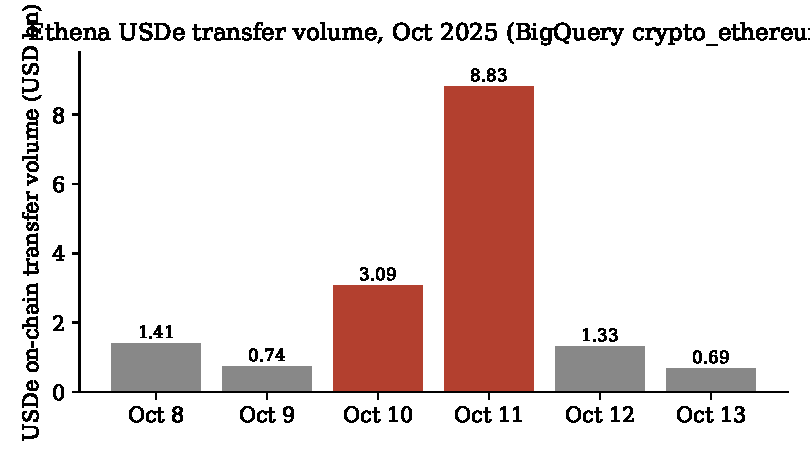
\includegraphics[width=\linewidth]{fig_usde_spike.pdf}
\end{minipage}\hfill
\begin{minipage}{0.62\linewidth}\centering
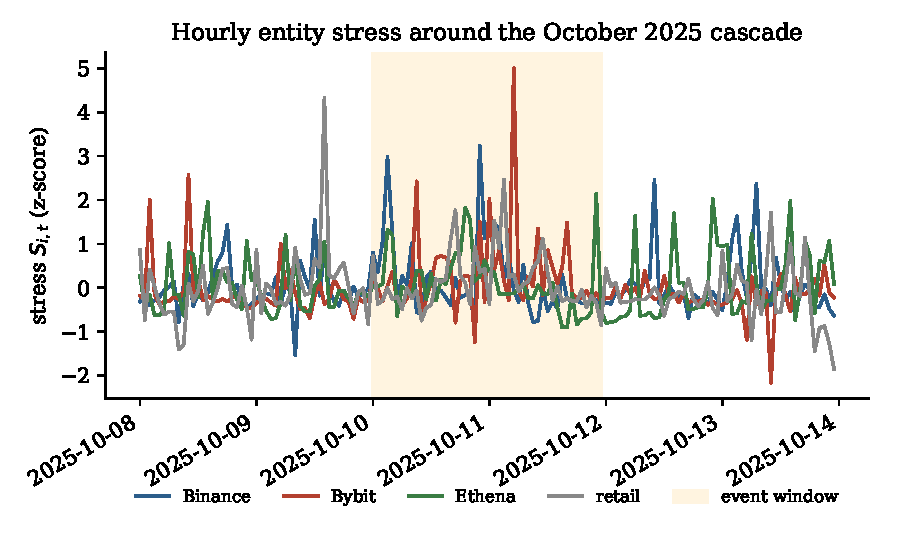
\includegraphics[width=\linewidth]{fig_stress.pdf}
\end{minipage}
\caption{Left: on-chain USDe transfer volume around the October~2025 cascade (BigQuery \texttt{crypto\_ethereum}
token transfers). Right: hourly stress $S_{i,t}$ of four entities, including
the peg component of the Ethena curve (shaded: the 10--11~October event window).}
\label{fig:usde}
\end{figure}

\subsection{Coverage and a data cross-check}
\label{subsec:coverage}
Named-to-named (distinct entities) flow is 3.0\% of entity-touching panel-token flow in October. Across
the six coverage extracts (the hourly, extended-window and daily builds) the range is 0.6--3.0\%. In the panel
that is actually fed to the model, named-to-named flow is 2.8\% of US\$570bn. The graph is therefore dominated by named-entity--retail edges.

As a cross-check, BigQuery daily USDe volume is compared with an earlier independent extraction. The two match within the
2\% tolerance on all six days, and the largest relative difference is 0.06\%. The volume peaks
at US\$3.09bn on 10~October and US\$8.83bn on 11~October.

\section{Empirical Evaluation}
\label{sec:results}

Unless noted, results are for the hourly October 2025 run (600 fitting hours, 48 event
hours, 15 entities, 90 directed edges). H1 and H2 are diagnostics,
and the numbers come from the \texttt{results/*.json} files named in the repository's numbers map. The daily specification
is used only for the analytic checks in Appendix~\ref{app:bounds}.

\subsection{How much stress does the network explain?}
\label{subsec:explained}
Table~\ref{tab:explained} reports in-sample and out-of-sample explained variance for each entity. In-sample $R^2$
ranges from 0.000 (Lido) to 0.273 (retail). Optimism-corrected, only retail
stays clearly above zero, at 0.186 [0.077, 0.265]. The Coinbase and Kraken intervals include
zero.

Out of sample, the network equation has pooled $R^2_{OS}=0.005$ [$-$0.017, 0.019], against
0.161 [0.056, 0.222] for the own lag. The network's squared-error gain over the own lag, $1-\mathrm{SSE}(m)/\mathrm{SSE}(\mathrm{AR})$, is $-$0.3\% [$-$2.0\%, 1.4\%] when added to the own lag and
$-$18.6\% [$-$27.1\%, $-$6.2\%] when used alone, so the network alone has larger error than the own lag. The large entity-level gains are for retail
(29.4\%) and Coinbase (11.6\%). The other entities lie between
$-$16.3\% and 1.6\%. Aave has the largest benchmark squared error, about 17.6\% of
the total, so it carries the most weight in the pooled score. Its own-lag $R^2_{OS}$ is 0.759. Pooled weights
follow benchmark squared error, so the equal-weight means are also reported: 0.081 for the own lag and
$-$0.003 for the network. The evidence rests on one window, two 24-hour blocks and one network specification.

\begin{lrbox}{\tabbox}\footnotesize\setlength{\tabcolsep}{3pt}%
\begin{tabular}{@{}lccccc@{}}
\toprule
\textbf{Entity} & \textbf{In-sample $R^2$} & \textbf{Optimism-corrected [95\% CI]} & \textbf{$R^2_{OS}$ AR} & \textbf{$R^2_{OS}$ network} & \textbf{AR+net vs AR (\%)}\\
\midrule
retail & 0.273 & 0.186 [0.077, 0.265] & 0.035 & 0.321 & 29.4 \\
Kraken & 0.140 & 0.050 [$-$0.157, 0.158] & 0.021 & $-$0.056 & $-$5.8 \\
Coinbase & 0.128 & 0.068 [$-$0.032, 0.131] & 0.022 & 0.053 & 11.6 \\
Binance & 0.061 & $-$0.008 [$-$0.089, 0.043] & 0.150 & 0.021 & $-$0.3 \\
Bitfinex & 0.052 & $-$0.006 [$-$0.116, 0.046] & $-$0.018 & $-$0.203 & $-$16.3 \\
Bybit & 0.048 & $-$0.014 [$-$0.109, 0.037] & $-$0.040 & $-$0.017 & $-$2.3 \\
OKX & 0.042 & 0.003 [$-$0.049, 0.038] & $-$0.004 & $-$0.108 & $-$11.0 \\
Crypto.com & 0.023 & $-$0.022 [$-$0.078, 0.017] & 0.007 & 0.016 & 1.6 \\
Ceffu & 0.021 & $-$0.043 [$-$0.237, 0.024] & $-$0.003 & $-$0.015 & $-$1.7 \\
HTX & 0.015 & $-$0.031 [$-$0.098, 0.008] & 0.000 & $-$0.120 & $-$12.1 \\
Aave & 0.014 & $-$0.041 [$-$0.150, 0.007] & 0.759 & 0.041 & $-$1.3 \\
Copper & 0.011 & 0.000 [$-$0.044, 0.016] & 0.033 & 0.023 & 0.9 \\
MakerSky & 0.011 & 0.001 [$-$0.034, 0.015] & 0.148 & $-$0.027 & $-$0.3 \\
Ethena & 0.001 & $-$0.015 [$-$0.047, $-$0.001] & 0.118 & 0.020 & 1.1 \\
Lido & 0.000 & $-$0.002 [$-$0.011, 0.000] & $-$0.005 & 0.000 & 0.0 \\
\midrule
Pooled (out of sample) & -- & -- & 0.161 & 0.005 & $-$0.3 \\
\bottomrule
\end{tabular}
\end{lrbox}
\begin{tableorg}[tbp]
\centering
\caption{Explained stress by entity, hourly October 2025. In-sample $R^2$ and its optimism-corrected value
with 95\% interval are from the bootstrap; out-of-sample $R^2_{OS}$ is from expanding-window one-step prediction.
Rows are sorted by in-sample $R^2$.}
\label{tab:explained}
\fitbox
\end{tableorg}

\subsection{Counterfactual attribution and the abduction lesson}
\label{subsec:attribution}
The largest share is 15.2\% [13.2\%, 19.5\%] (MakerSky$\to$retail; the interval is for the maximum over all pairs in each replicate, whereas the channel's own interval is in Table~\ref{tab:channels}). Of the ten largest channels
in the point estimate, four end at the retail aggregate, two start there, and four connect two named entities.
Table~\ref{tab:channels} reports the leading channels and Figure~\ref{fig:attribution} draws the top eight.

Among named-to-named channels, Binance$\to$Bybit has a share of 6.3\% [2.7\%, 8.6\%] with
$P(\text{attribution}>0)=1.00$. Crypto.com$\to$Binance (7.2\% [1.3\%, 12.5\%]) and
Binance$\to$OKX (6.7\% [0.4\%, 11.2\%]) have intervals above zero. The Kraken$\to$Bitfinex interval includes
zero (6.8\% [$-$9.2\%, 12.4\%]). The documented Ethena$\to$Aave$\to$Binance mechanism is not detected: Ethena$\to$Aave
is $-$1.1\% [$-$4.1\%, 2.3\%] and Ethena$\to$Binance is 0.4\% [$-$2.7\%, 3.2\%].

Table~\ref{tab:abduction} is the abduction lesson. Here v1 and v2 label earlier data builds (v2 is an earlier
BigQuery build) and v3 is the build used throughout this paper. On v1, zero-shock abduction gives a
Binance$\to$Bybit share of 98.1\% (L$_{\text{obs}}$ = 3.49). On the current data, the same
zero-shock abduction gives 65.3\% (L$_{\text{obs}}$ = 3.84), while full abduction gives
6.3\% (L$_{\text{obs}}$ = 21.66). The zero-shock share is inflated because its denominator is a
model-implied loss that omits the idiosyncratic shocks: Corollary~\ref{cor:share} and the Remark in
Section~\ref{subsec:risk} explain the mechanism. The zero-shock maximum over pairs is degenerate, with a tiny
denominator, and is not quoted. The v1 and v3 rows differ in data as well as in the
abduction mode, so only the same-data comparison isolates the abduction effect. Under full abduction the share is similar on the
v2 and v3 builds.

\begin{lrbox}{\tabbox}\footnotesize\setlength{\tabcolsep}{3pt}%
\begin{tabular}{@{}llccc@{}}
\toprule
\textbf{Data build} & \textbf{Abduction} & \textbf{$L_{\mathrm{obs}}$(Bybit)} & \textbf{Attribution} & \textbf{Share (\%)}\\
\midrule
v1 (earlier extract) & zero-shock & 3.49 & 3.42 & 98.1 \\
v3 (current build) & zero-shock & 3.84 & 2.51 & 65.3 \\
v3 (current build) & full & 21.66 & 1.37 & 6.3 \\
v2 (earlier BigQuery build) & full & 21.66 & 1.45 & 6.7 \\
\bottomrule
\end{tabular}
\end{lrbox}
\begin{tableorg}[tbp]
\centering
\caption{Abduction lesson for Binance$\to$Bybit. Attribution is the drop in Bybit's loss; the share is attribution
divided by $L_{\mathrm{obs}}$, which is the realised hinge loss under full abduction and the model-implied loss under zero-shock abduction.}
\label{tab:abduction}
\fitbox
\end{tableorg}

\begin{lrbox}{\tabbox}\footnotesize\setlength{\tabcolsep}{3pt}%
\begin{tabular}{@{}llcccc@{}}
\toprule
\textbf{Channel $i\!\to\! j$} & \textbf{Type} & \textbf{Attribution} & \textbf{Share (\%)} & \textbf{95\% CI of share (\%)} & \textbf{$P(\text{attribution}>0)$}\\
\midrule
MakerSky$\to$retail & $\to$retail & 2.19 & 15.2 & [12.2, 18.8] & 1.00 \\
Kraken$\to$retail & $\to$retail & 1.92 & 13.3 & [6.3, 19.0] & 1.00 \\
MakerSky$\to$Coinbase & named$\to$named & 1.34 & 10.9 & [7.7, 15.2] & 1.00 \\
Coinbase$\to$retail & $\to$retail & 1.48 & 10.3 & [5.7, 11.8] & 1.00 \\
retail$\to$Coinbase & retail$\to$ & 1.20 & 9.8 & [5.2, 15.1] & 1.00 \\
Bitfinex$\to$retail & $\to$retail & 1.31 & 9.1 & [2.7, 15.7] & 0.99 \\
retail$\to$OKX & retail$\to$ & 0.86 & 8.1 & [4.0, 11.2] & 1.00 \\
Crypto.com$\to$Binance & named$\to$named & 1.36 & 7.2 & [1.3, 12.5] & 0.99 \\
Kraken$\to$Bitfinex & named$\to$named & 0.61 & 6.8 & [$-$9.2, 12.4] & 0.87 \\
Binance$\to$OKX & named$\to$named & 0.72 & 6.7 & [0.4, 11.2] & 0.99 \\
\midrule
Binance$\to$Bybit & named$\to$named & 1.37 & 6.3 & [2.7, 8.6] & 1.00 \\
Ethena$\to$Aave & named$\to$named & $-$0.41 & $-$1.1 & [$-$4.1, 2.3] & 0.28 \\
Ethena$\to$Binance & named$\to$named & 0.08 & 0.4 & [$-$2.7, 3.2] & 0.59 \\
Lido$\to$Aave & named$\to$named & $-$0.01 & 0.0 & [$-$0.1, 0.0] & 0.12 \\
\bottomrule
\end{tabular}
\end{lrbox}
\begin{tableorg}[tbp]
\centering
\caption{Leading counterfactual loss-attribution channels $\Delta_i^{CF}(j)$, hourly October 2025. The top ten are chosen on the point
estimate, followed by four named-to-named channels. Intervals are not selection-adjusted. The maximum over all pairs is
15.2\% [13.2\%, 19.5\%].}
\label{tab:channels}
\fitbox
\end{tableorg}

\begin{figure}[tbp]
\centering
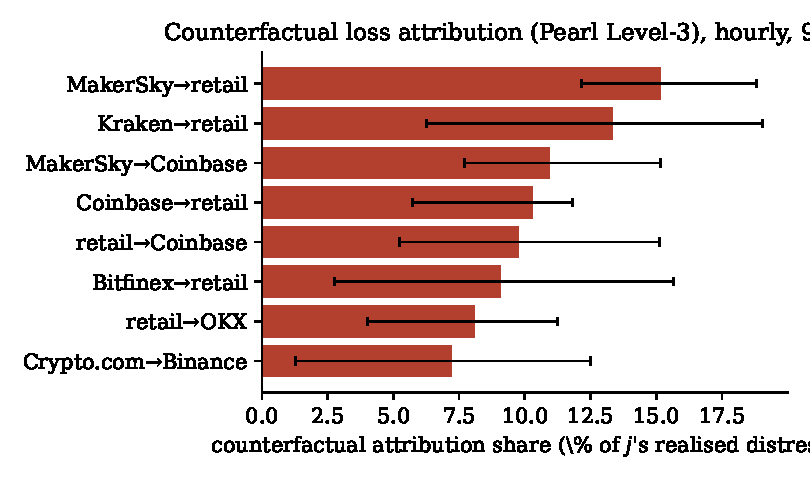
\includegraphics[width=0.70\linewidth]{fig_attribution.pdf}
\caption{Top eight counterfactual channels by point share, with 95\% bootstrap intervals (300 replicates). The intervals are not
selection-adjusted.}
\label{fig:attribution}
\end{figure}

For Bybit we also compute a Shapley decomposition of the hinge game over Binance, Coinbase and Bitfinex, by exhaustive
enumeration of the orderings. In this game the candidate set is held at its observed stress and every other entity at its
pre-crisis level, so only direct channels into Bybit operate. The values are Binance 1.49 [0.53, 2.00],
Coinbase 0.12 [$-$0.09, 0.24] and Bitfinex $-$0.37 [$-$0.97, 0.18]. They sum to the
total effect to machine precision (additive residual below $10^{-15}$). Only Binance's credit has an interval above zero.
This game differs from that of Proposition~\ref{prop:C}, which lets unselected entities propagate. The negative Bitfinex
value is therefore not the intermediary credit of Proposition~\ref{prop:C}. Its interval includes zero, so we do not trace
its source further.

\subsection{Systemic ranking with uncertainty}
\label{subsec:ranking}
Table~\ref{tab:rank} reports the ranking and Figure~\ref{fig:rank} reports the rank intervals and pairwise probabilities.
Retail and MakerSky are the top pair: $P(\text{top-3})=0.98$ for retail and $0.88$ for MakerSky. Their
order is unresolved, with $P(\text{retail above MakerSky})=0.80$. Ranks three to six are unresolved in
pairwise order, with pairwise probabilities between 0.34 and 0.66. Binance is ranked 7th, with rank interval [2, 9]. The five
lowest-ranked entities (ranks 11--15) all have $P(\text{top-5})=0$. The Spearman correlation between replicate and
point rankings is 0.903 [0.793, 0.968].

The retail aggregate matters for the ranking. Without retail, the ranking is led by Binance (17.67), Crypto.com
(14.81) and Kraken (14.33), and MakerSky drops out of the top six
(point estimates, no interval). Exported-risk levels scale with the number of entities, so only ranks
are comparable across runs.

\begin{lrbox}{\tabbox}\footnotesize\setlength{\tabcolsep}{3pt}%
\begin{tabular}{@{}llcccccc@{}}
\toprule
\textbf{Rank} & \textbf{Entity} & \textbf{Exported risk} & \textbf{MC s.e.} & \textbf{95\% CI of risk} & \textbf{Rank CI} & \textbf{$P(\text{top-1})$} & \textbf{$P(\text{top-3})$}\\
\midrule
1 & retail & 44.98 & 0.44 & [27.18, 75.19] & [1, 3] & 0.77 & 0.98 \\
2 & MakerSky & 37.89 & 0.29 & [23.70, 58.08] & [1, 5] & 0.17 & 0.88 \\
3 & Bitfinex & 26.20 & 0.32 & [8.89, 43.70] & [2, 10] & 0.02 & 0.24 \\
4 & Coinbase & 26.08 & 0.28 & [10.55, 45.96] & [1, 9] & 0.03 & 0.34 \\
5 & Kraken & 24.80 & 0.29 & [12.81, 41.64] & [2, 10] & 0.00 & 0.20 \\
6 & Crypto.com & 23.92 & 0.31 & [8.07, 45.43] & [2, 11] & 0.00 & 0.15 \\
7 & Binance & 22.35 & 0.30 & [12.06, 47.23] & [2, 9] & 0.00 & 0.17 \\
8 & OKX & 19.51 & 0.24 & [8.22, 34.16] & [3, 10] & 0.01 & 0.04 \\
9 & HTX & 13.68 & 0.25 & [3.97, 26.28] & [5, 12] & 0.00 & 0.00 \\
10 & Bybit & 13.43 & 0.20 & [3.25, 23.69] & [5, 13] & 0.00 & 0.00 \\
11 & Copper & 4.50 & 0.13 & [1.37, 13.83] & [9, 14] & 0.00 & 0.00 \\
12 & Aave & 3.38 & 0.12 & [0.08, 13.26] & [9, 15] & 0.00 & 0.00 \\
13 & Lido & 3.37 & 0.13 & [0.00, 9.26] & [10, 15] & 0.00 & 0.00 \\
14 & Ethena & 0.70 & 0.04 & [0.04, 7.57] & [11, 15] & 0.00 & 0.00 \\
15 & Ceffu & 0.55 & 0.02 & [0.00, 1.58] & [13, 15] & 0.00 & 0.00 \\
\bottomrule
\end{tabular}
\end{lrbox}
\begin{tableorg}[tbp]
\centering
\caption{Exported-risk ranking, hourly October 2025, with bootstrap intervals (300 replicates; the resolution of
$P(\cdot)$ is $1/300$). Rank intervals are percentile intervals. Spearman correlation between replicate and point
rankings: 0.903 [0.793, 0.968].}
\label{tab:rank}
\fitbox
\end{tableorg}

\begin{figure}[tbp]
\centering
\begin{minipage}{0.48\linewidth}\centering
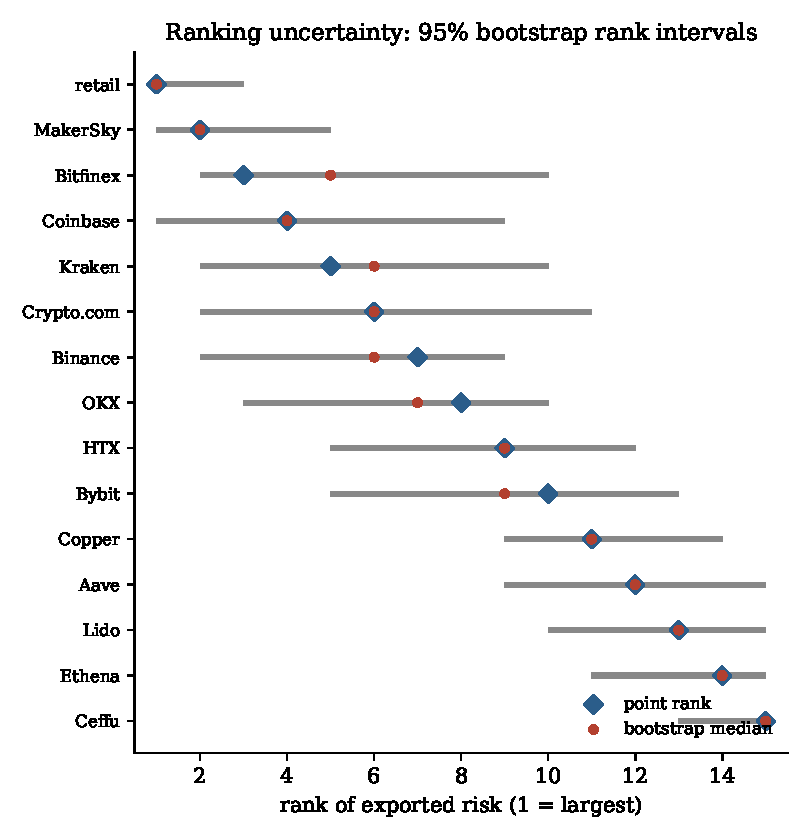
\includegraphics[width=\linewidth]{fig_rank_ci.pdf}
\end{minipage}\hfill
\begin{minipage}{0.48\linewidth}\centering
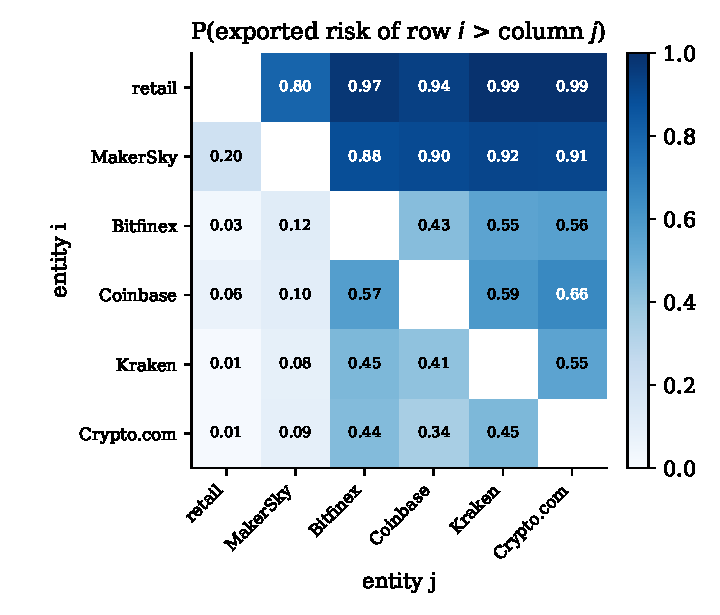
\includegraphics[width=\linewidth]{fig_pairwise_top6.pdf}
\end{minipage}
\caption{Left: rank intervals by entity. Right: pairwise order probabilities among the top six entities. Both use 300 refits.}
\label{fig:rank}
\end{figure}

\subsection{Graph source and direction diagnostics}
\label{subsec:diagnostics}
Table~\ref{tab:diagnostics} reports all comparisons. The H1 and H2 labels follow Section~\ref{subsec:design}.

\paragraph{H1: observed versus estimated graph.} The weighted RMSE is 1.5545 for the observed graph, 1.5595 for the
Granger graph and 1.5599 for the partial-correlation graph ($n=288$). The primary test uses unweighted squared error with
24-hour blocks. Its paired interval includes zero against both estimated graphs: the mean difference against Granger is
$-$0.0053 [$-$0.0129, 0.0021], and against partial correlation $-$0.0031 [$-$0.0151, 0.0094]. The
same holds with 8-hour blocks. In the weighted sensitivity test the Granger comparison is inconclusive, and against
partial correlation the interval only just excludes zero. Strictly lagged flows give the same picture
(weighted RMSE 1.5496 against 1.5571). The non-flow target and the daily H1 are omitted, since they share the
target and have low power. We conclude that H1 is not supported. The observed graph is not clearly better than the
estimated graphs.

\paragraph{H2: direction.} On the October run the true, reversed and symmetric graphs have RMSE 1.7841, 1.7871 and
1.7862. The reversed-minus-true interval is [$-$0.0006, 0.0093], which includes zero, as does the symmetric-minus-true
interval (Table~\ref{tab:diagnostics}). In the intraday A3 window, reversal is not distinguishable from the true graph
(interval [$-$0.0035, 0.0166]). The symmetric graph is worse than the true graph, with an interval [0.0003, 0.0250]
whose lower bound is barely above zero. Table~\ref{tab:diagnostics} contains ten uncorrected comparisons, and we do not read this one as evidence for
direction. For the two earlier episodes the direction results are inconclusive (Section~\ref{subsec:multievent}).
Splitting the October run by edge type, reversing the 86 custodial edges gives an RMSE of 1.7905, and reversing the
4 composability edges gives 1.7806 (true graph 1.7841). No intervals are computed for this split, and the
composability result rests on four edges. Direction is not distinguishable from reversal at the entity-aggregate hourly level.

\begin{lrbox}{\tabbox}\footnotesize\setlength{\tabcolsep}{3pt}%
\begin{tabular}{@{}llcccccl@{}}
\toprule
\textbf{Comparison} & \textbf{Window} & \textbf{$n$} & \textbf{RMSE base} & \textbf{RMSE alt} & \textbf{Mean diff} & \textbf{95\% CI} & \textbf{Status}\\
\midrule
H1: observed vs Granger & Oct 2025 & 288 & 1.5545 & 1.5595 & $-$0.0053 & [$-$0.0129, 0.0021] & inconclusive \\
H1: observed vs partial correlation & Oct 2025 & 288 & 1.5545 & 1.5599 & $-$0.0031 & [$-$0.0151, 0.0094] & inconclusive \\
\midrule
Reversed vs true & Oct 2025 & 720 & 1.7841 & 1.7871 & 0.0042 & [$-$0.0006, 0.0093] & inconclusive \\
Symmetric vs true & Oct 2025 & 720 & 1.7841 & 1.7862 & 0.0029 & [$-$0.0016, 0.0075] & inconclusive \\
\midrule
Reversed vs true & Intraday A3 & 720 & 1.8022 & 1.8036 & 0.0066 & [$-$0.0035, 0.0166] & inconclusive \\
Symmetric vs true & Intraday A3 & 720 & 1.8022 & 1.8097 & 0.0127 & [0.0003, 0.0250] & base better \\
\midrule
Reversed vs true & FTX, Nov 2022 & 1{,}344 & 1.3019 & 1.2987 & $-$0.0005 & [$-$0.0025, 0.0014] & inconclusive \\
Symmetric vs true & FTX, Nov 2022 & 1{,}344 & 1.3019 & 1.2995 & $-$0.0007 & [$-$0.0037, 0.0021] & inconclusive \\
Reversed vs true & USDC/SVB, Mar 2023 & 1{,}344 & 1.6514 & 1.6551 & 0.0033 & [$-$0.0026, 0.0113] & inconclusive \\
Symmetric vs true & USDC/SVB, Mar 2023 & 1{,}344 & 1.6514 & 1.6528 & 0.0024 & [$-$0.0011, 0.0064] & inconclusive \\
\bottomrule
\end{tabular}
\end{lrbox}
\begin{tableorg}[tbp]
\centering
\caption{Graph-source and direction comparisons. Mean difference is alternative minus base in squared error per entity-hour
cell (positive values favour the base). The RMSE columns are stress-weighted, whereas the mean difference and its interval use unweighted squared error, so their signs can differ. Base is the observed graph for H1 and the true-direction graph otherwise. Status is
the bootstrap verdict: base better (interval entirely above zero), alternative better (entirely below zero), or inconclusive.}
\label{tab:diagnostics}
\fitbox
\end{tableorg}

\subsection{Placebos and external validity}
\label{subsec:placebo}
The structural-zero check holds by construction: there are
196 connected and 14 unconnected pairs, and every unconnected pair has zero attribution. This is an
implementation check, not evidence. The rolling calm-window placebo gives $p=0.286$ over 20 windows, so it fails.
The time-shift placebo gives $p=0.0099$ (floor $1/(B+1)=0.0099$), so it passes ($B=100$ shifted refits, seed 11). The fitted network carries timing
information, but the event-window attribution is not unusual relative to calm windows. The FTX rolling placebo gives
$p=0.188$ (fails) and the SVB rolling placebo gives $p=0.032$ (passes). These are uncorrected.

External validity is checked by comparing transmitters (Ethena and Binance) with absorbers (Aave and Lido). Pairwise
concordance is 0.50 on the point estimate (0.65 averaged over the bootstrap replicates), and the separation is
8.15. The probability that all transmitters rank above all absorbers is 0.14. Binance passes the check, but Ethena fails
at rank 14. All four entities have non-degenerate stress, so the check is not vacuous.


\subsection{Multi-event validation}
\label{subsec:multievent}
We rerun the pipeline on two earlier episodes: the FTX collapse (event window 8--11 November 2022) and the USDC depeg
around the Silicon Valley Bank failure (event window 10--13 March 2023). These use the same CEX label set and the
hourly specification (Appendix~\ref{app:impl}). Table~\ref{tab:events} reports the top exporters, the rolling placebo and the direction verdict.

FTX is the top exporter, with rank interval [1, 3] and $P(\text{top-3})=1.00$. This is
consistent with the failing venue exporting stress, but it is descriptive: FTX's stress is flow-based and dominated by its own
outflows, and no causal claim is made. Retail is second and Binance third. In the SVB episode retail leads, followed by Binance and Coinbase.

Direction is inconclusive in both episodes. In FTX the reversed graph has the lowest RMSE, but the interval includes zero.
In SVB the true-direction graph has the lowest RMSE, the symmetric graph is close behind, and the reversed-minus-true interval includes zero. These comparisons are low-powered.
The earlier episodes have 912 and 888 fit rows, and the daily robustness runs have 38 and
37 fit rows against a required minimum of 125. The daily runs are therefore underpowered and are not reported.

\begin{lrbox}{\tabbox}\footnotesize\setlength{\tabcolsep}{3pt}%
\begin{tabular}{@{}lp{0.42\linewidth}ccc@{}}
\toprule
\textbf{Event} & \textbf{Top three exporters (rank CI; $P$(top-3))} & \textbf{Rolling $p$ (windows)} & \textbf{Reversed} & \textbf{Symmetric}\\
\midrule
Oct 2025 & retail rank [1, 3], $P$ = 0.98; MakerSky rank [1, 5], $P$ = 0.88; Bitfinex rank [2, 10], $P$ = 0.24 & 0.286 (20) & inconclusive & inconclusive \\
FTX, Nov 2022 & FTX rank [1, 3], $P$ = 1.00; retail rank [1, 3], $P$ = 0.98; Binance rank [2, 6], $P$ = 0.64 & 0.188 (31) & inconclusive & inconclusive \\
USDC/SVB, Mar 2023 & retail rank [1, 2], $P$ = 1.00; Binance rank [1, 5], $P$ = 0.85; Coinbase rank [2, 7], $P$ = 0.53 & 0.032 (30) & inconclusive & inconclusive \\
\bottomrule
\end{tabular}
\end{lrbox}
\begin{tableorg}[tbp]
\centering
\caption{Multi-event validation (hourly). Top three exporters with rank interval and $P(\text{top-3})$, the rolling
calm-window placebo $p$-value with the number of windows, and the direction verdict for reversal and symmetry.}
\label{tab:events}
\fitbox
\end{tableorg}

\subsection{Robustness}
\label{subsec:robustness}
The top-$k$, edge-dropping, latent-shock and coefficient-noise checks are point comparisons without bootstrap intervals
(\texttt{topk\_sensitivity.json}, \texttt{revision*.json}). The top-$k$ check compares the main specification with $k=10$ and $k=15$. The Spearman correlation over the common entities is
0.984 ($k=10$) and 0.986 ($k=15$), and the top-three overlap with the main run is 3 and 3 of three entities. The top channel,
MakerSky$\to$retail, has share 15.6\%, 15.2\% and 16.4\% at $k=10$, $12$ and $15$.

For confounding, the robustness values range from 0.089 to 0.231 across the 15 edges with the largest $t$-statistics of the 90 in the hourly graph, with
MakerSky$\to$retail at 0.231. These values are moderate, not large. Dropping the 22 lowest-RV edges leaves the Spearman
correlation at 0.989. A latent common shock of strength 0.3 and 0.6 gives Spearman correlations of 0.986 and 0.904,
with a mean top-three overlap fraction of 0.67. Coefficient noise (15\% relative standard deviation) changes the Binance$\to$Bybit share
by a standard deviation of 0.65 percentage points, and the share stays positive in every draw. The bootstrap width dominates.

Under the alternative resolution rule, the Spearman correlation with the main ranking is 0.714 over 6 common entities
(p=0.111), which is not established. For the price-based baseline, the Spearman correlation between the OC-CoVaR ranking and
$\Delta$CoVaR over six mapped entities is 0.371 (n=6). This is not distinguishable from zero, and is an illustration only.

\section{Discussion}
\label{sec:discussion}

\paragraph{What the ledger buys.} The observed transaction graph is auditable. Every edge maps to inspectable transfers, structural
zeros are exact, and attributions are reproducible from public data. It is not sufficient. At hourly scale the own lag and idiosyncratic
shocks account for more of stress than the network does, and the ledger-specified network adds nothing detectable out of sample.

\paragraph{Implications for supervisors and risk teams.} Ledger graphs are useful as an audit layer and a hypothesis generator, not as a
standalone contagion estimate. Any ``share of distress'' statement should use full abduction, because zero-shock abduction inflates
the Binance$\to$Bybit share from 6.3\% to 65.3\% on the same data. Explained-variance diagnostics should be
reported next to attributions, and rank uncertainty should be reported rather than point ranks.

\paragraph{Limits.} CEX opacity is the main threat to A2: the proximate cause, an exchange's pricing engine, is off-chain, and the
robustness values bound but cannot remove this threat. Label coverage is limited: named-to-named flow is about 3.0\% of
entity-touching flow, volume recall of the Tier-0 rule is at most 4.3\%, and validation covers only Binance and Bitget deposits.
The retail aggregate dominates both the ranking and the channels. The model is linear and has no own lag, and $s^\ast$ is held fixed
in the bootstrap. There are three events, and the tests are uncorrected for multiplicity. The DeFi nodes use price-based components.

\paragraph{Extensions.} Own-lag or regime-dependent structural equations, nonlinear clearing, intraday horizons, and better CEX resolution
are natural next steps.

\section{Conclusion}
\label{sec:conclusion}
We treat the entity-resolved on-chain ledger as a candidate structural skeleton. We give an interventional measure, OC-CoVaR, and a
counterfactual loss attribution with full abduction. We prove flow-free bounds, the network-multiplier form, abduction invariance of
the stress deviation, a share bound, the walk representation of the linear Shapley attribution and an exact subset algorithm. On the
October 2025 event the framework is auditable but explains little hourly stress out of sample, does not clearly beat price-estimated
graphs, and cannot identify edge direction. Its share-based statements are reliable only under full abduction and with
explained-variance diagnostics. The benchmark is released so that these conclusions can be checked on free public data.

\backmatter

\bmhead{Statements and Declarations}

\noindent\textbf{Data availability.} All code, query definitions and derived result files (\texttt{results/*.json}) underlying
every number, table and figure are available at [repository link withheld for review].
Raw transfers are not redistributed. They are regenerated from the public BigQuery dataset \texttt{bigquery-public-data.crypto\_ethereum}
(token transfers), which can be queried in the free BigQuery sandbox; the full build processed 327 GiB. Address labels come
from the eth-labels (commit \texttt{d9b21aefeded56f7fce7208d6fa173d128526c1b}) and etherscan-labels (commit \texttt{923aba72c7e2d0682f7ae6194b6140bd90668dc9}) repositories, both
MIT-licensed, and a label table built from these two sources alone is included. The Dune Spellbook CEX address list (commit
\texttt{6030202f2d6ee595dc568100c62723f26e5edda5}) is licensed under the Business Source License 1.1; it is fetched at the pinned commit at run time, used
only to build internal label tables, and is not redistributed. Prices are from CoinGecko and protocol TVL from DefiLlama. No
restricted or proprietary data were used.

\noindent\textbf{Code availability.} Code is in the repository named in the data availability statement.

\noindent\textbf{Ethics approval and consent to participate.} Not applicable: this study
uses only public, aggregated on-chain and market data and involves no human subjects.

\noindent\textbf{Consent for publication.} Not applicable.

\noindent\textbf{Competing interests.} The author declares no competing interests.

\noindent\textbf{Funding.} No external funding supported this work.

\noindent\textbf{Authors' contributions.} Withheld for review.

\begin{appendices}

\section{Implementation details and backtests}\label{app:impl}

The pipeline is implemented in Python, with on-chain data queried from BigQuery and cached by query hash. Structural equations
\eqref{eq:fi} are fitted by ridge regression with penalty $\lambda=1$. The deposit-sweep threshold is $\tau=0.8$, the VaR
level is $q=0.95$, and the seeds are $7$ for the point estimate, $20{,}251{,}010$ for the bootstrap, $20{,}251{,}011$ for the
attribution, and $11$ for the time-shift placebo. The Monte-Carlo point estimate uses 2{,}000 simulations, full abduction of
the event-window shocks, joint residual rows and the sample quantile $s^\ast=$ the 0.95 quantile of the fit window only
(600 hours). Each bootstrap replicate uses 500 simulations. The coefficient-perturbation checks multiply
every stress and flow coefficient by $1+\eta$ with $\eta\sim N(0,0.15^2)$. The H1 bootstrap uses $B=2{,}000$ circular blocks.

\section{Entity-resolution validation}\label{app:resolution}

Table~\ref{tab:tier0} reports the Tier-0 validation per extract. The Tier-0 rule is the deposit-sweep rule of
Section~\ref{subsec:resolution}, with the tightened parameters used only for FTX.

\begin{lrbox}{\tabbox}\footnotesize\setlength{\tabcolsep}{3pt}%
\begin{tabular}{@{}lllcccccc@{}}
\toprule
\textbf{Extract} & \textbf{Rule} & \textbf{$\tau$} & \textbf{Holdout} & \textbf{Overlap} & \textbf{Wrong root} & \textbf{Precision} & \textbf{Recall (count)} & \textbf{Recall (volume)}\\
\midrule
Oct 2025 (hourly) & default & 0.8 & 25{,}080 & 423 & 0 & 1.00 & 68.3 & 0.4 \\
FTX (hourly) & tightened & 0.9 & 25{,}080 & 13 & 0 & 1.00 & 17.1 & 4.3 \\
USDC/SVB (hourly) & default & 0.8 & 25{,}080 & 31 & 0 & 1.00 & 34.1 & 3.2 \\
Daily core & default & 0.8 & 25{,}080 & 64 & 0 & 1.00 & 55.2 & 0.1 \\
\bottomrule
\end{tabular}
\end{lrbox}
\begin{tableorg}[tbp]
\centering
\caption{Tier-0 validation against the holdout deposit labels. Recall by count and by volume and the precision are for the chosen rule.}
\label{tab:tier0}
\fitbox
\end{tableorg}

The Tier-1 classifier and the embedding are validated against CEX-labelled addresses in the USDe window
(8--14~October 2025). After the mint/burn sentinel is excluded, the window has 7{,}019 addresses, of which 41 are CEX-labelled
(base rate 0.6\%). The held-out ROC-AUC is 0.89, and the average precision is 0.17. At the best-$F_1$
threshold the classifier's precision and recall by address count are 0.13 and 0.58. By USD volume, precision is
0.92 and recall is only 0.15. The Tier-2 cluster homogeneity is 0.10.
The ground truth is small and deposit-dominated, so these numbers are a weak check. Tier-3 label matching therefore remains the
production resolver.

\section{Proofs}\label{app:proofs}

Let $h(y)=\max(y,0)$, which is nondecreasing and 1-Lipschitz, so $\min(\delta,0)\le h(x+\delta)-h(x)\le\max(\delta,0)$.

\noindent\textbf{Proof of Proposition~\ref{prop:A}.} (a) Let $D_t=S^{(s)}_t-S^{(0)}_t$.
Both paths share the initial state and the inputs $\kappa$, so $D_{-1}=0$. For $j\neq i$,
$D_{j,t}=\sum_p a_{jp}D_{p,t-1}$. For $i$, $D_{i,t}=s$ for $t<T$. We show $D_t=s\tau_t$ by
induction. At $t=0$, $D_0=se_i=s\tau_0$. For $t\ge1$, the $j\neq i$ coordinates satisfy
$D_{j,t}=s\sum_pa_{jp}\tau_{p}(t-1)=s\,(A\tau_{t-1})_j=s\,\tau_j(t)$, since the reset
affects only the $i$-th coordinate, and $D_{i,t}=s=s\,\tau_i(t)$.

(b) For a fixed realisation let $x_t=S^{(0)}_{j,t}$. Then $L_j^{(s)}-L_j^{(0)}=\sum_{t<T}[h(x_t+s\tau_{ji}(t))-h(x_t)]$, and each summand lies in $[\min(s\tau_{ji}(t),0),\max(s\tau_{ji}(t),0)]$. The sums $\ell$ and $u$ of these endpoints are deterministic, so $L_j^{(0)}+\ell\le L_j^{(s)}\le L_j^{(0)}+u$ pointwise. Quantiles are monotone and translation-equivariant, which gives $\VaR_q(L^{(0)}_j)+\ell\le\VaR_q(L^{(s)}_j)\le\VaR_q(L^{(0)}_j)+u$, and the same holds for the Monte-Carlo estimator with shared draws. \hfill$\square$

\noindent\textbf{Proof of Corollary~\ref{cor:zero}.} The induction in the text shows that $\tau_{ji}(t)\neq0$ requires a directed path from $i$ to $j$ of length at most $t$. Without such a path, $\tau_{ji}(t)=0$ on the window and Corollary~\ref{cor:pure} gives $\Delta\OCCoVaR_q(j\,|\,i)=0$. For the attribution, $r_j\equiv0$ in Proposition~\ref{prop:B} with $K=\{i\}$, so \eqref{eq:cfhinge} gives $\Delta_i^{CF}(j)=0$. \hfill$\square$

\noindent\textbf{Proof of Corollary~\ref{cor:bound}.} (i) The upper bound in Proposition~\ref{prop:A}(b) is non-negative for $s>0$, so
$\max(\Delta\OCCoVaR_q(j|i),0)\le s\sum_t\max(\tau_{ji}(t),0)$. Summing over $j\neq i$ gives $\mathcal{E}(i)\le s\Lambda_i(T)$.
So $\Lambda_i(T)=0$ forces $\mathcal{E}(i)=0$.
(ii) For $t\ge1$, $x_t=\tau_{\cdot i}(t)$ restricted to $V\setminus\{i\}$ satisfies $x_t=A'x_{t-1}+b$, with $A'=A_{-i,-i}$, $b=A_{-i,i}$, $x_0=0$.
With $m=(I-A')^{-1}b$ and $\rho(A')<1$, we have $x_t-m=A'^t(x_0-m)\to0$. The Cesàro mean of the
convergent sequence $\max(x_t,0)$ converges to $\max(m,0)$, which gives the limit of
$\Lambda_i(T)/T$. \hfill$\square$

\noindent\textbf{Proof of Proposition~\ref{prop:B}.} Let $D=S^K-S^{\mathrm f}$. Both paths
share the inputs $\kappa$ and the initial state, so $D_{-1}=0$. For $k\in K$,
$D_{k,t}=p_{k,t}-S^{\mathrm f}_{k,t}=-g_{k,t}$. For $j\notin K$, both paths satisfy
\eqref{eq:linear}, so $D_{j,t}=\sum_pa_{jp}D_{p,t-1}$. Induction on $t$ shows $D=-r$, since
$r$ satisfies the same recursion with the same forcing. Hence $S^K=S^{\mathrm f}-r(K)$.
Taking $K=\{i\}$ and $p_{i,t}\equiv S_i^{\mathrm{pre}}$ gives $L_j^{\doop}=\sum_t\max(S^{\mathrm f}_{j,t}-r_{j,t}(\{i\}),0)$,
and \eqref{eq:cfhinge} follows from $\Delta_i^{CF}(j)=L_j^{\mathrm{fact}}-L_j^{\doop}$. \hfill$\square$

\noindent\textbf{Proof of Proposition~\ref{prop:C}.} (a) Unrolling the recursion for $r$ backwards from $(j,t)$, a node in $K$ stops the recursion as a forcing term and a node outside $K$ passes it to its parents. Hence $r_{j,t}(K)$ is the sum of $\omega(w)$ over walks from a forced node $x_0\in K$ whose intermediate nodes avoid $K$, which is the indicator in (a). Walks that revisit $x_0$ contain $x_0\in K$ among their intermediates and are excluded by the same condition, so restricting to $\mathcal W$ changes nothing.

(b) By linearity it suffices to treat $u_w(K)=\mathbf 1[x_0\in K,\ I(w)\cap K=\emptyset]$. Let
$k=x_0$, $I=I(w)$, $m=|I|$, and let $\mathrm{Pre}_y$ be the players preceding $y$ in a uniformly
random ordering; the Shapley value of $y$ is its expected marginal contribution. For $y=k$ the
marginal is $\mathbf 1[\mathrm{Pre}_k\cap I=\emptyset]$, and $k$ precedes all of $I$ with
probability $1/(m+1)$. For $y\in I$ the marginal is $-\mathbf 1[k\in\mathrm{Pre}_y,\ \mathrm{Pre}_y\cap I=\emptyset]$.
This requires $k$ to be first and $y$ second among $\{k\}\cup I$, which has probability
$1/((m+1)m)$. For any other $y$ the game does not depend on $y$. This gives
$\phi_k(u_w)=1/(1+m)$, $\phi_y(u_w)=-1/(m(m+1))$ for $y\in I$, and zero otherwise. Summing
over walks with the weights $\omega(w)$ gives \eqref{eq:phi}.

(c) Summing \eqref{eq:phi} over $k\in P$ gives $\omega(w)[\tfrac1{1+m}-\tfrac1{m+1}]=0$ for $m\ge1$ and $\omega(w)$ for $m=0$, which matches (a) at $K=P$.

(d) If $S^{\mathrm f}_{j,t}\ge0$ and $S^{\mathrm f}_{j,t}-r_{j,t}(K)\ge0$, then both hinge terms are linear, so
$v_H(K)=v(K)$. \hfill$\square$

\begin{lemma}[Certified ranking radius]
\label{lem:radius}
Let $\tilde A$ satisfy $|\tilde a_{jp}-a_{jp}|\le\varepsilon|a_{jp}|$ with the same sparsity
pattern, and let $\tilde\Lambda_i$ be $\Lambda_i(T)$ computed from $\tilde A$. Then
$|\tilde\Lambda_i-\Lambda_i(T)|\le R_i(\varepsilon)$, where
$R_i(\varepsilon)=\sum_{j\ne i}\sum_{t<T}\big[\tau^{(1+\varepsilon)|A|}_{ji}(t)-\tau^{|A|}_{ji}(t)\big]$.
If $\Lambda_r-\Lambda_{r+1}>R_r(\varepsilon)+R_{r+1}(\varepsilon)$, the order of the pair is
preserved under every such perturbation.
\end{lemma}
\begin{proof}
$\tau_{ji}(t)$ is a sum over walks from $i$ to $j$ of length at most $t$ avoiding $i$ in between. The telescoping bound $|\prod\tilde a_e-\prod a_e|\le\prod(1+\varepsilon)|a_e|-\prod|a_e|$ gives the entrywise bound, and $h$ is 1-Lipschitz.
\end{proof}

\section{Daily analytic checks and bounds}\label{app:bounds}
\setcounter{table}{0}

The numbers come from \texttt{results/analytics.json}, which uses the daily SCM with $T=7$ and 15 entities; the
spectral radius is $\rho(A)=0.569$. $B^+$ is $\Lambda_i(T)$ per unit $s^\ast$ (Corollary~\ref{cor:bound}), so the stored
exported risk must satisfy $\mathcal{E}(i)\le s^\ast B^+$, and the implied minimum $s^\ast$ is $\mathcal{E}/B^+$. The
infinite-horizon multiplier is a reference quantity, not a bound. These checks were not
run on the hourly coefficients, which are archived in \texttt{hourly\_scm\_export.json}.

There are 0 violations of the bound. 5 entities have $B^+=0$ and stored $\mathcal{E}=0$; the bound is vacuous for them
because their coefficients are all zero. This is a one-directional sanity check, not out-of-sample validation. Table~\ref{tab:bounds} lists the bounded entities; the other 5 have $B^+=0$. Coefficients are archived to four decimals, so the implied minimum
$s^\ast$ values are approximate.

The certified ranking radius (Lemma~\ref{lem:radius}) applies to the ranking by $\Lambda_i(T)$ under relative coefficient
perturbations of size $\varepsilon$. For the top five daily entities (retail, Aave, Lido, MakerSky and Copper), the certified radii
for consecutive pairs are 0.047, 0.064, 0.134 and 0.305, and no pair is certified at $\varepsilon=1$.
The certificate does not cover the exported-risk ranking $\mathcal{E}$, flows, shocks, $s^\ast$ or estimation error.

The closed-form walk decomposition agrees with subset enumeration to within $10^{-15}$ on a synthetic deviation path (seed
7), and the subset and permutation computations agree to the same precision. Subset enumeration needs 8{,}192 oracle calls
against 80{,}951{,}270{,}400 for permutations at $p=13$, the retail parent set. The exact subset computation for retail took 0.22 s on one machine.

\begin{lrbox}{\tabbox}\footnotesize\setlength{\tabcolsep}{3pt}%
\begin{tabular}{@{}lcccc@{}}
\toprule
\textbf{Entity} & \textbf{Stored $\mathcal{E}$} & \textbf{$B^+$ per unit $s^\ast$} & \textbf{Implied min.\ $s^\ast$} & \textbf{$\infty$-horizon multiplier}\\
\midrule
retail & 8.284 & 4.414 & 1.88 & 0.737 \\
Lido & 6.678 & 3.151 & 2.12 & 0.675 \\
Aave & 6.457 & 3.906 & 1.65 & 0.682 \\
MakerSky & 1.161 & 1.780 & 0.65 & 0.373 \\
Ethena & 0.041 & 0.243 & 0.17 & 0.041 \\
Bybit & 0.024 & 0.034 & 0.70 & 0.007 \\
Ceffu & 0.019 & 0.037 & 0.52 & 0.009 \\
Copper & 0.002 & 0.365 & 0.00 & 0.061 \\
Binance & 0.001 & 0.005 & 0.28 & 0.001 \\
FalconX & 0.000 & 0.058 & 0.00 & 0.014 \\
\bottomrule
\end{tabular}
\end{lrbox}
\begin{tableorg}[tbp]
\centering
\caption{Flow-free bounds on exported risk, daily specification ($T=7$), bounded entities only.}
\label{tab:bounds}
\fitbox
\end{tableorg}

\end{appendices}

{\footnotesize\linespread{1.05}\selectfont
\bibliography{references}}

\end{document}
